\chapter{Sorting algorithms}
\label{app:sorting} This section will explain some of the sorting algorithms that are used in some of the papers mentioned in chapter \ref{sec:background}. 
\section{Odd even sort}
Odd even sort is a sorting algorithm which resembles bubble sort. The algorithm takes a list of elements, then compares all the odd placed element with the element next to it. That is; compare list[i] with list[i+1] where $i$ is an odd number. Then the algorithm does the same for all $i$ even number. This is done repeatedly until we get a sorted list.

\section{Bitonic sort}
Bitonic sort is a highly parallel sorting algorithm, the idea is to have the elements in the list in a bitonic sequence. A bitonic sequence is a sequence where the list is increasing, then decreasing and then eventually increasing again. However the last increasing part are not allowed to increase past the first element in the list.
\begin{figure}[H]
    \centering
    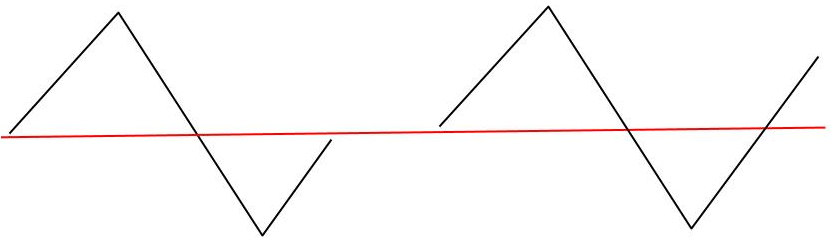
\includegraphics[width=0.8\linewidth]{images/bitonicseq}
    \caption[Sequence of elements]{Left figure is a bitonic sequence, right figure is not a bitonic sequence because the last increasing part is higher than the start}\label{fig:bitonicseq}
\end{figure}
After the algorithm have obtained a bitonic sequence, it will start to compare the elements with certain distance from each other and swap these elements if they are in the wrong order.
\begin{figure}[H]
    \centering
    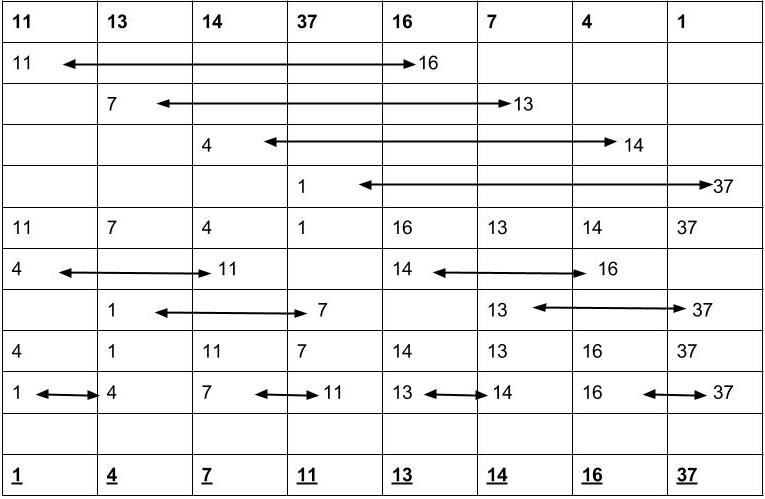
\includegraphics[width=0.8\linewidth]{images/bitonicexample}
    \caption{Example of a bitonic sort run}\label{fig:bitonicex}
\end{figure}
In the example we have the numbers 11,13,14,37,16,7,4,1. Which is initially in a bitonic sequence because the first half is increasing and the last half is decreasing. The algorithm now compares the first and the fifth element, as indicated by the arrows. All of these comparisons can be done in parallel. The algorithm compares the elements at different position, in the example it start with a comparison of elements that are distance 4 away from each other, that is element at position 1 and 5, 2 and 6 and so on. Then elements with distance 2 is compared, and then elements with distance 1 are compared.
The runtime of the bitonic sort algorithm is $O(nlog(n)^2)$ but the idea is to run it on $n$ Cuda threads, reducing the runtime to $O(log(n)^2)$ for each thread.
